\documentclass[usenames,dvipsnames, 9pt]{beamer}
\usepackage{amsmath,amsfonts,amssymb}
\usepackage{mathtools}
\usepackage{etex} %for Windows
\usepackage[utf8]{inputenc}
\usepackage[english, russian]{babel} 

%\usepackage{microtype}			% Better interword spacing and additional kerning.
\usepackage{ellipsis}			% Adjusted space with \dots between two words.
\usepackage{graphicx}
\usepackage{pstricks}

\usepackage{xcolor}


\usepackage{changepage}

\usepackage{algorithm}
\usepackage{algpseudocode}
%\usepackage[]{algorithm2e}
%\usepackage{algorithmic}

%\usepackage{tcolorbox}






\usepackage{tikz}
\usetikzlibrary{tikzmark,calc}
\usetikzlibrary{positioning, backgrounds}
\usetikzlibrary{arrows, chains, matrix, scopes, patterns, shapes, fit}
\usetikzlibrary{mindmap,trees,shadows}
\usetikzlibrary{decorations.pathreplacing}

\usepackage{pgfplots}

\pgfmathdeclarefunction{gauss}{2}{%
	\pgfmathparse{1/(#2*sqrt(2*pi))*exp(-((x-#1)^2)/(2*#2^2))}%
}


\tikzset{
	invisible/.style={opacity=0},
	visible on/.style={alt={#1{}{invisible}}},
	alt/.code args={<#1>#2#3}{%
		\alt<#1>{\pgfkeysalso{#2}}{\pgfkeysalso{#3}} % \pgfkeysalso doesn't change the path
	},
}

\newcommand\strikeout[2][]{%
	\begin{tabular}[b]{@{}c@{}} 
		\makebox(0,0)[cb]{{#1}} \\[-0.2\normalbaselineskip]
		\rlap{\color{Orange}\rule[0.5ex]{\widthof{#2}}{1.5pt}}#2
\end{tabular}}

\newcommand\Fontvi{\fontsize{11}{13.2}\selectfont}

\usepackage{listings} % for C++ code

\usepackage{braket}
%\usepackage[braket, qm]{qcircuit}



\usepackage[T1]{fontenc}
%\usepackage[sfdefault,scaled=.85]{FiraSans}
%\usepackage{newtxsf}
%\usepackage[nomap]{FiraMono}





\usefonttheme[onlymath]{serif}
\renewcommand\sfdefault{cmbr}

\renewcommand{\bfdefault}{sb}




\definecolor{CharCoalDark}{RGB}{13, 16, 19}
\definecolor{Orange}{RGB}{255, 165,0}
\definecolor{DarkOrange}{RGB}{255, 165,0}
\definecolor{LightSalmon}{RGB}{255, 160, 122}
\definecolor{LeafGreen}{RGB}{34, 139,  34}
\definecolor{Coral}{RGB}{255, 127, 80}
\definecolor{DarkTurquoise}{RGB}{0, 206, 209}

%\newtheorem{defRus}{Определение}
%\newtheorem{thmRus}{Теорема}
%s\newtheorem{corRus}{Следствие}


\setbeamercolor{background canvas}{bg=CharCoalDark}

\setbeamerfont{title}{series=\bfseries}
\setbeamercolor{title}{fg=Orange}
\setbeamercolor{section in toc}{fg=white}
\setbeamercolor{frametitle}{fg=Orange}
\setbeamercolor{normal text}{fg=white}
%\setbeamercolor{normal text}{fontsize=12pt}
\setbeamercolor{itemize item}{fg=Orange}
\setbeamercolor{itemize item item}{fg=Orange}
\setbeamercolor{enumerate item}{fg=Orange}
\setbeamercolor{block title}{bg=DarkOrange,fg=white}
\setbeamerfont{block title}{series=\bfseries}

\setbeamertemplate{itemize item}[circle]
%\setbeamertemplate{itemize subitem}[$\checkmark$]
%\setbeamertemplate{itemize subitem}{\color{Orange}\Large${\checkmark}$}
\setbeamertemplate{itemize subitem}{\color{Orange}\Large $\blacksquare$}

% footnote without a marker
\newcommand\blfootnote[1]{%
	\begingroup
	\renewcommand\footnoterule{}
	\renewcommand\thefootnote{}\footnote{#1}%
	\addtocounter{footnote}{-1}%
	\endgroup
}

\newcommand*{\Scale}[2][4]{\scalebox{#1}{\ensuremath{#2}}}%


\AtBeginSection[]
{
	\begin{frame}<beamer>
		\frametitle{Outline}
		\tableofcontents[currentsection]
	\end{frame}
}


%\institute{ENS Lyon}
\author{Елена Киршанова \\ [10pt]
	%based on joint works with G.Herold, T.Laarhoven
}
\titlegraphic{
	%\includegraphics[width=2.5cm]{erc_logo_gray}\hspace*{2.5cm}~%
	\hspace*{1.0cm}
\includegraphics[width=4.0cm]{GC_BFU_logo_full_cyr_bw}
}
\title{ Алгоритм Просеивания для решения задачи SVP}

\date{ Курс ``Криптография на решетках''  \\ \today }


\setbeamertemplate{navigation symbols}{} %removes navigation

% proper highlightling of a code-snippet
\lstset{language=C++,
	keywordstyle=\color{magenta},
	stringstyle=\color{Goldenrod},
	commentstyle=\color{gray},
	breaklines=false,
	%morecomment=[l][\color{magenta}]{\#}
}

\setlength{\parskip}{8pt}

% ==================================================================
% Definitions for this paper
% ==================================================================
\mathchardef\hyphen="2D

\usepackage{multirow}
\usepackage{multicol} % For multiple coloumn environments
%\usepackage{stmaryrd} % For set brackets
% \setlength{\columnsep}{15pt} % Defining the coloumn seperation
% \setlength{\columnseprule}{1pt} % Place a line between coloumns
% \newcommand{\tab}{\hspace*{2em}}

%subscripts

\newcommand*\SmallTextScript[2]{{\mathchoice{\displaystyle #2}
		{\textstyle #2}%dito
		{\scalebox{#1}{\ensuremath{\scriptstyle #2}}}%
		{\scalebox{#1}{\ensuremath{\scriptscriptstyle #2}}}%
}}


% ADVERSARIES AND SUCH
\newcommand*{\poly}{\ensuremath{\mathrm{poly}}}
\newcommand*{\eps}{\ensuremath{\varepsilon}}
\newcommand*{\alg}{\ensuremath{\mathcal{A}}}

% GROUPS/DISTRIBUTIONS/SETS/LISTS
\newcommand{\N}{{{\mathbb N}}}
\newcommand{\Z}{{{\mathbb Z}}}
\newcommand*{\IZ}{\ensuremath{\mathbb{Z}}}
\newcommand*{\IN}{\ensuremath{\mathbb{N}}}
\newcommand*{\IQ}{\ensuremath{\mathbb{Q}}}
\newcommand{\R}{{{\mathbb R}}}
\newcommand*{\IR}{{{\mathbb R}}}
\newcommand{\Zp}{\ints_p} % Integers modulo p
\newcommand{\Zq}{\ints_q} % Integers modulo q
\newcommand{\Zn}{\ints_N} % Integers modulo N
\newcommand{\F}{\ensuremath{\mathbb{F}}}
\newcommand{\CC}{\ensuremath{\mathbb{C}}}

\newcommand{\GF}{\ensuremath{\mathbb{F}_2}}
\newcommand{\GFn}{\ensuremath{\mathbb{F}^n_2}}

%%% ALGORITHMS/PROCEDURES %%%
\newcommand{\Dec}{\textsf{Dec}}
\newcommand{\Enc}{\textsf{Enc}}
\newcommand{\KeyGen}{\textsf{KeyGen}}
\newcommand{\Gen}{\textsf{Gen}}
\newcommand{\sk}{\textsf{sk}}
\newcommand{\pk}{\textsf{pk}}
\newcommand{\vk}{\textsf{vk}}
\newcommand{\mesS}{\ensuremath{\mathcal{M}}}
\newcommand{\keyS}{\ensuremath{\mathcal{K}}}
\newcommand{\cipS}{\ensuremath{\mathcal{C}}}
\newcommand{\tagS}{\ensuremath{\mathcal{T}}}
\newcommand{\mactag}{\textsf{tag}}
\newcommand{\Hash}{\ensuremath{\mathcal{H}}}
\newcommand{\EID}{\ensuremath{\mathtt{EphID}}}


\newcommand{\adv}{\ensuremath{\mathcal{A}}}

\newcommand{\LWE}{\mathsf{LWE}}
\newcommand{\DCP}{\mathsf{DCP}}
\newcommand{\EDCP}{\mathsf{EDCP}}
\newcommand{\UEDCP}{\mathsf{U \text{-} EDCP}}
\newcommand{\GEDCP}{\mathsf{G \text{-} EDCP}}



%% Landau and proba
\newcommand{\bigO}{\mathcal{O}}
\newcommand*{\OLandau}{\bigO}
\newcommand*{\WLandau}{\Omega}
\newcommand*{\xOLandau}{\widetilde{\OLandau}}
\newcommand*{\xWLandau}{\widetilde{\WLandau}}
\newcommand*{\TLandau}{\Theta}
\newcommand*{\xTLandau}{\widetilde{\TLandau}}
\newcommand{\smallo}{o} %technically, an omicron
\newcommand{\wLandau}{\omega}
\newcommand{\negl}{\mathrm{negl}}
\newcommand*\PROB\Pr 
\DeclareMathOperator*{\EXPECT}{\mathbb{E}}
\DeclareMathOperator*{\VARIANCE}{\mathbb{V}}
\DeclareMathOperator*{\LOGBIAS}{\mathbb{LB}}

\newcommand{\supp}{\ensuremath{\mathsf{sup}}}
\newcommand{\Distr}{\ensuremath{\mathcal{D}}}

% Lattices

% \newcommand{\coset}{\Lambda} % Lambda Lattice
% \newcommand{\cosetPerp}{\Lambda^{\bot}} % Lambda_Perp Lattice
% \newcommand{\gadget}{\textbf{G}} %Gaget matrix
% \newcommand{\mes}{\textbf{m}} %message vector
% \newcommand{\AMat}{\textbf{A}} %A matrices
% \newcommand{\BMat}{\textbf{B}} %B matrices
% \newcommand{\RMat}{\textbf{R}} %R matrices
% \newcommand{\HMat}{\textbf{H}} %H matrices
% \newcommand{\XMat}{\textbf{X}} %H matrices
% \newcommand{\mbar}{\bar{m}} %mBar dimension
% % \newcommand{\gauss}{\mathcal{D}} % gaussian distribution
% \newcommand{\Id}{\textbf{I}} % Identity matrix
% \newcommand{\er}{\textbf{e}} % gaussian distr. vectors
% % \newcommand{\cipher}{\textit{c}} % ciphertext
% \newcommand{\Olwe}{\mathcal{O}_{\textsf{LWE}}} %LWE oracle
% \newcommand{\OSample}{\mathcal{O}_{Sample}} %LWE oracle
% \newcommand{\SigmaB}{\boldsymbol{\Sigma}} %semi-deifinite matrix Sigma%
% % \newcommand{\mods}{\text{ mod}}


%Vectors and Matrices

\newcommand{\AMat}{\mathbf{A}} %A matrices
\newcommand{\BMat}{\mathbf{B}} %B matrices
\newcommand{\DMat}{\mathbf{D}} %Diagonal


\newcommand{\HMat}{\ensuremath{\mathbf{H}}}
\newcommand{\QMat}{\ensuremath{\mathbf{Q}}}
\newcommand{\Id}{\ensuremath{\mathbf{I}}}
\newcommand{\ZeroM}{\textbf{0}} % Zero matrix

\newcommand{\avec}{\ensuremath{\mathbf{a}}}
\newcommand{\bvec}{\ensuremath{\mathbf{b}}}
\newcommand{\cvec}{\ensuremath{\mathbf{c}}}
\newcommand{\evec}{\ensuremath{\mathbf{e}}}
\newcommand{\rvec}{\ensuremath{\mathbf{r}}}
\newcommand{\svec}{\ensuremath{\mathbf{s}}}
\newcommand{\tvec}{\ensuremath{\mathbf{t}}}
\newcommand{\vvec}{\ensuremath{\mathbf{v}}}
\newcommand{\zvec}{\ensuremath{\mathbf{z}}}
\newcommand{\xvec}{\ensuremath{\mathbf{x}}}
\newcommand{\yvec}{\ensuremath{\mathbf{y}}}
\newcommand{\uvec}{\ensuremath{\mathbf{u}}}
\newcommand{\zerovec}{\ensuremath{\mathbf{0}}}

\newcommand{\nth}{^{\mathrm{th}}}
\newcommand{\nd}{^{\mathrm{nd}}}

\newcommand{\RepMMT}{\ensuremath{\mathcal{R}_{\protect\SmallTextScript{0.70}{\texttt{MMT}}}}}
\newcommand{\RepBJMM}{\ensuremath{\mathcal{R}_{\protect\SmallTextScript{0.70}{\texttt{BJMM}}}}}
\newcommand{\XOR}{\ensuremath{\mathtt{3XOR}}}


% % % % % \newcommand{\mb}[1]{\mathbf{#1}} % does not compile otherwise
%%% Removed by Gotti; this is just asking to screw up with packages that (properly) define \mb (mathbold)

% \newcommand{\bL}{\|\bvec_1\|} % b1 length that appears way too often
% \newcommand{\dL}{\|\dvec_1\|} % b1 length that appears way too oftend

%Norms and Scalar products

\newcommand*\abs[1]{\left\lvert#1\right\rvert}
\newcommand*\norm[1]{\left\lVert#1\right\rVert}
\newcommand*\normalabs[1]{\lvert#1\rvert} 
\newcommand*\normalnorm[1]{\lVert#1\rVert}
\newcommand*\bignorm[1]{\bigl\lVert#1\bigr\rVert}
\newcommand*\bigabs[1]{\bigl\lvert#1\bigr\rvert}
\newcommand*\Bigabs[1]{\Bigl\lvert#1\Bigr\rvert}
\newcommand*{\ScProd}[2]{\ensuremath{\langle#1\mathbin{,}#2\rangle}} %Scalar Product
% \newcommand*{\ScProd}[2]{\ensuremath{\langle#1 \:{,}\:#2\rangle}} %Scalar Product
\newcommand*{\bigScProd}[2]{\ensuremath{\bigl\langle#1\mathbin{,}#2\bigr\rangle}} %Scalar Product
\newcommand*{\BigScProd}[2]{\ensuremath{\Bigl\langle#1\mathbin{,}#2\Bigr\rangle}} %Scalar Product
\newcommand{\dist}{\ensuremath{\text{dist}}}


%Some other math operators

\DeclareMathOperator{\Span}{Span} %span of vectors
\DeclareMathOperator{\vol}{\mathrm{vol}} %volume
\DeclareMathOperator{\LW}{LambertW} %Lambert W function
\DeclareMathOperator{\SD}{SD}
\DeclareMathOperator{\gradient}{grad}
\DeclareMathOperator{\TRACE}{Tr}
\newcommand*{\dDR}{\mathrm{d}} %de-Rham-Differential (the d in dx, dy, dz and so on)


%Lists
\renewcommand{\L}{\ensuremath{\mathcal{L}}}

\renewcommand{\P}{\ensuremath{\mathcal{P}}}

\newcommand*{\Lout}{\ensuremath{\L_{\mkern-0.5mu\protect\SmallTextScript{0.85}{\textup{out}}}}}
\newcommand*{\Sout}{\ensuremath{S_{\mkern-0.5mu\protect\SmallTextScript{0.85}{\textup{out}}}}}
\newcommand{\wt}{\ensuremath{\mathit{wt}}}


\newcommand*{\softO}{\widetilde{\bigO}}

\newcommand{\const}{\mathsf{c}} 


\newcommand{\transpose}{\mkern0.7mu^{\mathsf{ t}}}

%proper overline reduced by 1.5mu
\newcommand{\overbar}[1]{\mkern 1.5mu\overline{\mkern-1.5mu#1\mkern-1.5mu}\mkern 1.5mu}

\DeclareMathOperator{\erf}{erf} %error function
\DeclareMathOperator{\erfc}{erfc} %complementary error function
\newcommand{\Er}{\ensuremath{\mathrm{Er}}} %complementary error function


% LATTICES

\newcommand{\Lat}{\ensuremath{\mathcal{L}}}
\newcommand*{\Sphere}[1]{\ensuremath{\mathsf{S}^{#1}}}
%\DeclareMathOperator{\Conf}{Conf}
\newcommand{\Conf}{\mathcal{C}}

%Thick line for table
\setlength{\doublerulesep}{0pt}
\newcommand{\thickline}{\hline\hline\hline}


%circled text
\newcommand*\circled[1]{\tikz[baseline=(char.base)]{
    \node[shape=circle,draw,inner sep=0.3 pt] (char) {\scriptsize #1};}}


%Fix Algorithmicx package
\def\NoNumber#1{{\def\alglinenumber##1{}\State #1}\addtocounter{ALG@line}{-1}}

%For comments
\newcommand{\GColor}{ForestGreen}  %Damiens' color
\newcommand{\EColor}{MidnightBlue} %Elena's color

\newcommand*{\E}[1]{{\color{\EColor} #1} } 
\newcommand*{\G}[1]{{\color{\GColor} #1} } 

%Proper limit with the subscript underneath
% \newcommand{\Lim}[1]{\raisebox{0.5ex}{\scalebox{0.8}{$\displaystyle \lim_{#1}\;$}}}


%TIKZ dense dotted pattern

\pgfdeclarepatternformonly{my dots}{\pgfqpoint{-1pt}{-1pt}}{\pgfqpoint{2.0pt}{2.0pt}}{\pgfqpoint{2pt}{2pt}}%
{
	\pgfpathcircle{\pgfqpoint{0pt}{0pt}}{.35pt}
	\pgfpathcircle{\pgfqpoint{1pt}{1pt}}{.35pt}
	\pgfusepath{fill}
}


\tikzset{
	master/.style={
		execute at end picture={
			\coordinate (lower right) at (current bounding box.south east);
			\coordinate (upper left) at (current bounding box.north west);
		}
	},
	slave/.style={
		execute at end picture={
			\pgfresetboundingbox
			\path  (lower right)rectangle (upper left) ;
		}
	}
} %all defs
\begin{document}
	
\begin{frame}
	\titlepage
\end{frame}

%\begin{frame}{Outline}
%	\tableofcontents
%\end{frame}






\begin{frame}{Поиск кратчайшего вектора \\ \underline{S}hortest\underline{V}ector\underline{P}roblem}
\vspace{-15pt}
\begin{tikzpicture}%[show background grid]
\hspace{-30pt}
\begin{scope}
\foreach \y in {-2,...,3}
\foreach \x in {-2,...,3}
\filldraw(\x*40pt+\y*10pt, 10pt*\x+20pt*\y) circle (1.7pt);

\filldraw(0pt,0pt) circle (1.7pt) node[below]{ $0$};

\draw[-stealth, white, thick] (0,0) -- (50pt, 30pt) node[font=\Large, above, xshift=5pt]{$\bvec_1$};
\draw[-stealth, white, thick] (0,0) -- (40pt, 10pt) node[font=\Large, below, xshift=5pt]{$\bvec_2$};

\draw[-stealth, Orange, thick] (0, 0) -- (10pt, 20pt) node[font=\LARGE, left]{$\vvec$};

%	\draw[fill=CharCoalDark, draw=none, opacity=0.5] (3.2,-2.0) rectangle (8.5,4.0) node[color=white, opacity=1,align=center] at (6.2, 3.0){
%	
%	\Large  {\color{Orange}{\underline{Minimum}} }  \\[3pt]
%	\Huge	$\lambda_1(\Lat) = \min_{\substack{\vvec \in \Lat \setminus \zerovec}} \norm{\vvec} $ \\[10pt]
%};
%
%\draw[fill=CharCoalDark, draw=none, opacity=0.5] (3.2,0.0) rectangle (8.5,2.0) node[color=white, opacity=1,align=center] at (6.2, 1.0){
%	\Large  {\color{Orange}{\underline{Determinant}} }  \\[3pt]
%	\Huge	$\det(\Lat) = \abs{\det(\bvec_i)_i}$ \\[10pt]
%};
%
%\draw[fill=CharCoalDark, draw=none, opacity=0.5] (3.2,-2.0) rectangle (8.5,0.0) node[color=white, opacity=1,align=center] at (6.2, -1.0){
%	\Large  {\color{Orange}{\underline{Minkowski bound}} }  \\[3pt]
%	\Huge	$\lambda_1(\Lat) \leq \sqrt{n} (\det(\Lat))^{\frac{1}{n}}$ \\[3pt]
	
%}; 

\end{scope}
\end{tikzpicture}
\vspace{-15pt}
\Large {
	
	B  {\color{Orange}{задаче поиска кратчайшего вектора} (SVP)} требуется найти $\vvec_{\text{shortest}} \in \Lat$: 
	\[
		\norm{\vvec_{\text{shortest}}} = \lambda_1(\Lat)
	\]
	\pause
	Упрощение: поиск {\color{Orange} аппроксимации ($\gamma$-SVP)} к $\vvec_{\text{shortest}}$:
	\[
		||\vvec_{\text{short}}||  \leq {\color{Orange} \gamma} \cdot \lambda_1(\Lat) 
	\]
}
\end{frame}

\begin{frame}{Поиск ближайшего вектора {\textbf{C}}VP / BDD}
\vspace{-30pt}
\begin{tikzpicture}%[show background grid]
\hspace{-30pt}
\begin{scope}
\foreach \y in {-2,...,4}
\foreach \x in {-2,...,3}
\filldraw(\x*40pt+\y*10pt, 10pt*\x+20pt*\y) circle (1.7pt);

\filldraw(0pt,0pt) circle (1.7pt) node[below]{ $0$};

\draw[-stealth, white, thick] (0,0) -- (50pt, 30pt) node[font=\Large, above, xshift=5pt]{$\bvec_1$};
\draw[-stealth, white, thick] (0,0) -- (40pt, 10pt) node[font=\Large, below, xshift=5pt]{$\bvec_2$};

%\draw[-stealth, Orange, thick] (0, 0) -- (10pt, 20pt) node[font=\LARGE, left]{$\vvec$};

\filldraw[fill=Orange, draw=Orange](-18pt,45pt) circle (1.7pt) node[below right, yshift=3pt, xshift=-2pt]{ \LARGE $\tvec$};
\draw[fill=none, draw=Orange] (-18pt,45pt) circle (10pt);
\filldraw(-10pt,50pt) circle (1.7pt) node[below right]{ \Large $\vvec$};
\onslide<3->
{
\draw[fill=CharCoalDark, draw=none, opacity=0.5] (2.2,-3.0) rectangle (8.5,3.0) node[color=white, opacity=1,align=center] at (6.2, 1.0){
	\LARGE 
	Для решения BDD в $\Lat$, \\[3pt]
	\LARGE
	вызываем оракул для approx-SVP на \\[3pt]
	\LARGE
	``связанной'' решетке р-ти+1. \\[3pt]
};
}

\end{scope}
\end{tikzpicture}
	\vspace{-25pt}
\Large {

	В задаче {\color{Orange}{поиска ближайшего вектора} (CVP)} для $\tvec \notin \Lat$ требуется найти $\vvec \in \L$:
	\[
	\norm{\vvec - \tvec} \text{минимально для всех } \vvec \in \Lat
	\]
	\pause
	Часто: $\dist(t, \Lat) \leq \frac{1}{\gamma} \lambda_1(\Lat)$. 
	Получаем задачу {\color{Orange}Декодирования с Ограниченным расстоянием,  $\gamma$-BDD}
	
}
\end{frame}	



\begin{frame}{Асимптотическая сложность SVP \small ($\smallo()$ опущены)}
\LARGE
\vspace{-30pt}
\begin{align*}
||\vvec_{\text{shortest}}|| & \leq \sqrt{n} \cdot \det(\L)^{1/n}  \hspace{80pt} \\[5pt]
||\vvec_{\text{short}}|| & \leq {\color{Orange} \gamma} \cdot \norm{\vvec_{\text{shortest}}}
\end{align*}	

	\vspace{-10pt}
	\begin{tikzpicture}
	
	\draw[-stealth, white, thick] (0,0) -- (10.5, 0) node[font=\Large, below, yshift=-5pt]{\huge \color{Orange} $\mathbf{\gamma}$} node[above, yshift=4pt]{Время};
	
	\draw[-] (0.5,-0.3) -- (0.5,0.3) node[above, xshift=7pt] {\texttt{NP}-hard} node[below, yshift=-20pt, align=left, xshift=7pt] {\huge $2^{\log^{1-\eps} n}$};
	
	\draw[-] (2.8,-0.3) -- (2.8,0.3) node[above, xshift=10pt, align=center] {\LARGE $2^{\const  \cdot n}$ or \LARGE $2^{\const  \cdot n \log n}$ } node[below, yshift=-20pt, align=center, xshift=7pt] {$\poly(n)$ \\ (Крипто)};
	
	\draw[-] (5.5,-0.3) -- (5.5,0.3) node[above] {\LARGE $ 2^{\beta}$, \texttt{BKZ}} node[below, yshift=-20pt, align=left, xshift=4pt] {\huge $2^{ \tfrac{n}{\beta} \log \beta} $};
	
	\draw[-] (8.5,-0.3) -- (8.5,0.3) node[above] {$\poly(n)$, \texttt{LLL}} node[below, yshift=-20pt, align=left, xshift=4pt] {\huge $2^{\tfrac{n\log \log n}{\log n}}$};    
	
	\pause
	\onslide<2->{
		\draw[draw=Orange, very thick] (1.7, -2.0) rectangle (4.4, 1.5);
	}
	\end{tikzpicture}
	\vspace{-20pt}
	\onslide<2->{
	\begin{itemize}
		\item {\color{Orange}Просеивание} (эвристический): $\text{Время({exactSVP})} = 2^{ 0.292n}
		\quad \quad \quad \hspace{10pt}\text{Память} = 2^{ 0.2075n} $
		\item {\color{Orange}Перечисление:} $\text{Время({exactSVP})} = 2^{ (1/2e)n \log n}
		\quad \quad \text{Память} = \poly(n)$
	\end{itemize}
}
\end{frame}

\begin{frame}{Алгоритмы для SVP}
\renewcommand{\arraystretch}{1.5}
\begin{table}[h]
	\centering
	\begin{tabular}{| l | c | c |}
		\hline
		\textbf{Алгоритм} & \textbf{Время} & \textbf{Память} \\ \hline
		\multicolumn{3}{|c|}{\textsc{ Детерминированные алгоритмы:} } \\ \hline
		Перечисление & $n^{ (1/2e) n + \smallo(n)}$ & $\poly(n)$ \\ \hline
		Диаграмма Вороного & $2^{2n + \smallo(n)}$ & $2^{n+\smallo(n)}$ \\ \hline
		\multicolumn{3}{|c|}{\textsc{ Вероятностные алгоритмы:} } \\ \hline
		Гауссова выборка  & $2^{n+ \smallo(n)}$ & $2^{n+ \smallo(n)}$ \\ \hline
		Просеивание & & \\ [-1ex]
		\hspace{5pt} -- С док-вом  & $2^{2.465n + \smallo(n)}$& $2^{1.325n + \smallo(n)}$ \\ [-1ex]
		\hspace{5pt} -- Эвристические: & & \\ [-1ex]
		\hspace{15pt} -- $2$-просеивание  & $2^{0.415 n + \smallo(n)}$ & $2^{0.208n + \smallo(n)}$\\
		\hspace{15pt} -- $2$-просеивание+LSH  & $2^{0.415 n + \smallo(n)}$ & $2^{0.208n + \smallo(n)}$\\
		\hspace{15pt} -- $3$-просеивание & $2^{0.396n + \smallo(n)}$ & $2^{0.1887n + \smallo(n)}$  \\ \hline
		
	\end{tabular}
\end{table}

\end{frame}

\begin{frame}
\renewcommand\footnoterule{}
\begin{center}
	
	Часть II \\ [10pt]
	
	\color{Orange}
	\Huge{Алгоритмы просеивания}
	
	\vspace{10pt}
	
	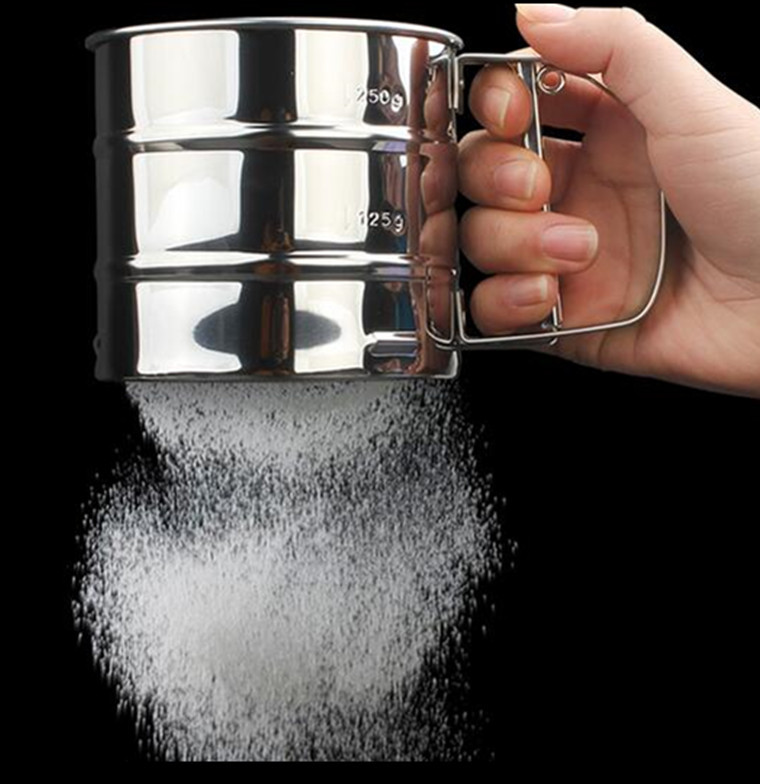
\includegraphics[width=4.0cm]{siever.jpg}
	\blfootnote{{\color{gray}https://sites.google.com/a/x.bestledlights.cf/a223/1-32772214555}}
\end{center}
\end{frame}

\begin{frame}{2-Просеивание (Nguyen-Vidick)}
\vspace{-5pt}
\Large
{\color{Orange}Идея:} {\color{Orange} насыщать} пространство векторами решётки так, чтобы суммы их пар давали короткие вектора
\begin{tabular}{@{}c @{}c }
	\hspace{-30pt}
	\begin{tikzpicture}
	%\vspace*{-50pt}
	\centering
	\onslide<1->{
		\draw[rounded corners, thick] (0pt, 0pt) rectangle (30pt, 50pt) node(L1)[xshift=-15pt, below]{\Large $L$};
		\draw[rounded corners, thick] (40pt, 0pt) rectangle (70pt, 50pt)node(L2)[xshift=-15pt, below]{\Large $L$};
		\node[draw=none] at (35pt, 35pt){$=$};
	}
	\pause
	\onslide<3->{
		\draw[rounded corners, thick] (20pt, -60pt) rectangle (50pt, -10pt) node(L3)[xshift=-15pt, below]{\Large $L'$};
		
		\draw[-] ([yshift=-37pt]L1.south) -- (L3.north) node[left, xshift=-16pt,yshift=-10pt, align=left]{\Large $\xvec_1 \pm \xvec_2$ \\[3pt] $||\xvec_1 \pm \xvec_2||$\\[3pt]-- мало};
		\draw[-] ([yshift=-37pt]L2.south) -- (L3.north);
	}
	\pause
	
	\onslide<4->{
		\draw[rounded corners, thick] (60pt, -60pt) rectangle (90pt, -10pt) node(L4)[xshift=-15pt, below]{\Large $L'$};
		\node[draw=none] at (55pt, -20pt){$=$};
	}
	\pause
	\onslide<5->
	{
		\draw[-] ([yshift=-37pt]L3.south) -- (55pt, -68pt) node[below]{$\vdots$} node[right, yshift=-5pt]{$\poly(n)$};
		\draw[-] ([yshift=-37pt]L4.south) -- (55pt, -68pt);
	}
	
	%\onslide<4>{
	%	\node[below, text width=3.5cm, xshift=5cm] at (85pt,10pt) {Memory: $2^{\bigO(n)}$};
	%}
	
	%\pause
	%\node[below, text width=3.5cm, xshift=5cm, font=\bfseries, color=red] at (85pt,10pt) {Memory: $2^{\bigO(n)}$};
	\end{tikzpicture} &
	\begin{tikzpicture}
	%\begin{scope}
	\onslide<1->{
		\clip (10pt,50pt) circle (100pt);
		\foreach \y in {-3,...,6}
		\foreach \x in {-5,...,5}
		\filldraw[gray!70](\x*40pt+\y*10pt, 10pt*\x+20pt*\y) circle (1.5pt);
		
		\filldraw(0pt,0pt) circle (1pt) node[below] (zero) { $0$};
	}
	
	\onslide<1-2>{
		\filldraw[orange!70](-40pt, 60pt) circle(2.0pt) node (v1) {};
		\filldraw[orange!70](-10pt, 50pt) circle(2.0pt) node (v2) {};
		\filldraw[orange!70](-70pt, 70pt) circle(2.0pt) node (v3) {};
		\filldraw[orange!70](-60pt, 20pt) circle(2.0pt) node (v4) {};
		
		\filldraw[orange!70](60pt, 50pt) circle(2.0pt) node (v5) {};
		\filldraw[orange!70](100pt, 60pt) circle(2.0pt) node (v6) {};
		
		%\filldraw(50pt, 100pt) circle(1.3pt) node (v7) {};
		%\filldraw(40pt, 80pt) circle(1.3pt) node (v8) {};
	}
	
	\onslide<2>{
		\draw[-stealth, thick] (v1) -- (v2);
		\draw[-stealth, thick] (v1) -- (v3);
		\draw[-stealth, thick] (v1) -- (v4);
		
		\draw[dashed] ([shift=({-5pt,-10pt})]v1) circle (38pt);
		
		\draw[-stealth, thick] (v5) -- (v6);
		\draw[dashed] ([shift=({-5pt,-10pt})]v6) circle (38pt);
		
		%\draw[->, thick] (v8) -- (v7);
		%\draw[dashed] ([shift=({-20pt,5pt})]v7) circle (38pt);
	}
	
	\onslide<3->{
		\filldraw[orange!70](30pt, -10pt) circle(1.5pt) node (v1v2){};
		\filldraw[orange!70](-30pt, 10pt) circle(1.5pt) node (v1v3){};
		\filldraw[orange!70](-20pt, -40pt) circle(1.5pt) node (v1v4){};
		
		\filldraw[orange!70](40pt, 10pt) circle(1.5pt) node (v5v6){};
		
		%\filldraw[orange!70](10pt, 20pt) circle(1.5pt) node (v7v8){};
		
		\draw[-stealth, thick] (zero.north) -- (v1v2);
		\draw[-stealth, thick] (zero.north) -- (v1v3);
		\draw[-stealth, thick] (zero.north) -- (v1v4);
		
		\draw[-stealth, thick] (zero.north) -- (v5v6);
	}
	
	\onslide<3>{
		\filldraw[orange!70](30pt, -10pt) circle(1.5pt) node (v1v2){};
		\filldraw[orange!70](-30pt, 10pt) circle(1.5pt) node (v1v3){};
		\filldraw[orange!70](-20pt, -40pt) circle(1.5pt) node (v1v4){};
		
		\filldraw[orange!70](40pt, 10pt) circle(1.5pt) node (v5v6){};
		
		%\filldraw[orange!70](10pt, 20pt) circle(1.5pt) node (v7v8){};	
		
		\draw[dashed] ([shift=({6pt,-8pt})]zero.north)  circle (42pt);
	}
	\onslide<5->{
		%\filldraw[red!80]  circle(1.5pt)  {};
		\draw[-stealth, thick, red!80] (30pt, -10pt) -- (40pt, 10pt);
	}
	
	%		\onslide<6->
	%		{
	%			\draw[draw=CharCoalDark,fill=CharCoalDark] (-2.6,1.0) rectangle (4,3.0) node[pos=0.5, color=white,align=left]{
	%							 \Huge $|L| = \softO(  2^{0.2075n} )$ \\ [7pt]
	%							 \Huge $T(\text{\Large naive 2-Sieve}) =\softO( |L|^2)$
	%			};
	%		}
	%\end{scope}
	\end{tikzpicture}
\end{tabular}
\end{frame}

\begin{frame}{Насколько большим должно быть $|L|$?}
\pause
Предположение: вектора (нормализованные) в $|L|$ равномерно независимо распределены в $S^{n-1}$. \\

\tikzmark{start}
\includegraphics[width=\textwidth]{semi-sphere1}
\tikzmark{end}
\end{frame}
\begin{frame}{Насколько большим должно быть $|L|$?}
Предположение: вектора (нормализованные) в $|L|$ равномерно независимо распределены в $S^{n-1}$. \\

\tikzmark{start}
\includegraphics[width=\textwidth]{semi-sphere2}
\tikzmark{end}
\end{frame}

\begin{frame}{ 2-Просеивание (Nguyen-Vidick)}
\vspace{-5pt}
\Large
{\color{Orange}Идея}: {\color{Orange} насыщать} пространство векторами решётки так, чтобы суммы их пар давали короткие вектора
\begin{tabular}{@{}c @{}c }
\hspace{-30pt}
\begin{tikzpicture}
%\vspace*{-50pt}
\centering
\draw[rounded corners, thick] (0pt, 0pt) rectangle (30pt, 50pt) node(L1)[xshift=-15pt, below]{\Large $L$};
\draw[rounded corners, thick] (40pt, 0pt) rectangle (70pt, 50pt)node(L2)[xshift=-15pt, below]{\Large $L$};
\node[draw=none] at (35pt, 35pt){$=$};

\draw[rounded corners, thick] (20pt, -60pt) rectangle (50pt, -10pt) node(L3)[xshift=-15pt, below]{\Large $L'$};

\draw[-] ([yshift=-37pt]L1.south) -- (L3.north) node[left, xshift=-16pt,yshift=-10pt, align=left]{\Large $\xvec_1 \pm \xvec_2$ \\[3pt] $||\xvec_1 \pm \xvec_2||$\\[3pt] -- мало};

\draw[rounded corners, thick] (60pt, -60pt) rectangle (90pt, -10pt) node(L4)[xshift=-15pt, below]{\Large $L'$};
\node[draw=none] at (55pt, -20pt){$=$};

\draw[-] ([yshift=-37pt]L3.south) -- (55pt, -68pt) node[below]{$\vdots$} node[right, yshift=-5pt]{$\poly(n)$};
\draw[-] ([yshift=-37pt]L4.south) -- (55pt, -68pt);

\end{tikzpicture} &
\begin{tikzpicture}

\clip (10pt,50pt) circle (100pt);
\foreach \y in {-3,...,6}
\foreach \x in {-5,...,5}
\filldraw[gray!70](\x*40pt+\y*10pt, 10pt*\x+20pt*\y) circle (1.5pt);

\filldraw(0pt,0pt) circle (1pt) node[below] (zero) { $0$};


\filldraw[orange!70](30pt, -10pt) circle(1.5pt) node (v1v2){};
\filldraw[orange!70](-30pt, 10pt) circle(1.5pt) node (v1v3){};
\filldraw[orange!70](-20pt, -40pt) circle(1.5pt) node (v1v4){};

\filldraw[orange!70](40pt, 10pt) circle(1.5pt) node (v5v6){};

\filldraw[orange!70](10pt, 20pt) circle(1.5pt) node (v7v8){};	


\draw[-stealth, thick, red!80] (30pt, -10pt) -- (40pt, 10pt);

\draw[draw=CharCoalDark,fill=CharCoalDark] (-3.0,-1.0) rectangle (4,3.0) node[pos=0.5, color=white,align=left]{
\Huge
$
\begin{aligned}
\Huge |L| = \left(\sqrt{\frac{3}{4}}\right)^{-n} \mkern-15mu &= 2^{0.2075n} \\
\Huge T(\text{\Large 2-Просеивания}) & =|L|^2 \\
& = 2^{0.415n} \blfootnote{ \smallo(n) опушены}
\end{aligned}
$
};
%\end{scope}
\end{tikzpicture}
\end{tabular}
\end{frame}
%\Huge $|L| = \left(\sqrt{\frac{3}{4}}\right)^{-n} \mkern-15mu =   
%2^{0.2075n} $ \\ [7pt]
%\Huge $T(\text{\Large naive 2-Sieve}) =\softO( |L|^2)$ \\
\begin{frame}{Улучшенное просеивание с хэшированием}
\LARGE
\begin{center}
Как достичь $T =2^{0.292n + \smallo(n)}? $ \\[10pt]

Использовать метод "Ближнего соседа" (Near Neighbour)!\\
(aka Locality-Sensitive techniques)
\end{center}
\pause

\begin{align*}
||\xvec_1 - \xvec_2|| &< ||\xvec_1||  \iff \\
||\xvec_1 - \xvec_2||^2 &< ||\xvec_1|| ^2 \iff \\
||\xvec_1||^2 - 2 \langle \xvec_1, \xvec_2 \rangle + ||\xvec_2||^2 &< ||\xvec_1|| ^2 \iff \\
\langle \xvec_1, \xvec_2 \rangle &> \frac{1}{2} ||\xvec_2||^2
\end{align*}

\end{frame}

\begin{frame}{Locality-sensitive filtering (Фильтрация по расстоянию) [BGJ15, BDGL16]}
\tikzmark{start}
\includegraphics[width=\textwidth]{LSF_explained}
\tikzmark{end}
\end{frame}

\begin{frame}{Locality-sensitive filtering (Фильтрация по расстоянию)[BGJ15, BDGL16]}
\tikzmark{start}
\includegraphics[width=\textwidth]{LSF_explained_2}
\tikzmark{end}
\end{frame}

%\begin{frame}{Locality-sensitive filtering (Фильтрация по расстоянию)[BGJ15, BDGL16]}
%\tikzmark{start}
%\includegraphics[width=\textwidth]{LSF_explained_2_2}
%\tikzmark{end}
%\end{frame}

\begin{frame}{Locality-sensitive filtering (Фильтрация по расстоянию)[BGJ15, BDGL16]}
\tikzmark{start}
\includegraphics[width=\textwidth]{LSF_explained_2}
\tikzmark{end}
\begin{tikzpicture}[remember picture,overlay]
\centering
%\onslide<1->{
\draw[draw=none] (1.0,7.5) rectangle (2.0, 8.5) node[pos=.5, color=white, align=left]{ 
\LARGE  $u_i$ -- центры "корзин" \\ [4pt] \LARGE $x_i \in L$};

\onslide<2->
{
\draw[fill=CharCoalDark] (-0.8,6) rectangle (6.0,9) node[pos=.5, color=white, opacity=0.7,align=left]{ \LARGE
For all $\uvec_i:$\\ [4pt]
\LARGE
\hspace{8pt} For all $\xvec \in L$  \\[4pt]
\LARGE
\hspace{18pt} If $\abs{\langle \xvec, \uvec_i \rangle}$ достаточно велико \\[4pt]
\LARGE
\hspace{26pt} добавить $\xvec$ в $\texttt{Bucket}(\uvec_i)$ 
};
}
\onslide<3->
{
\draw[fill=CharCoalDark] (-0.8,2.5) rectangle (6.0,5.5) node[pos=.5, color=white, opacity=0.7,align=left]{ \LARGE
For all $\uvec_i:$\\ [4pt]
\LARGE
\hspace{8pt} For all $(\xvec, \xvec') \in \texttt{Bucket}(\uvec_i)$  \\[4pt]
\LARGE
\hspace{18pt} Проверить если $||\xvec \pm \xvec'||$ -- мало

};
}
\onslide<4->
{
\draw[fill=CharCoalDark] (6.3,2.5) rectangle (11.4,9) node[pos=.5, color=white, opacity=0.7,align=center]{ \LARGE
Для $2^{(0.142+\smallo(1)) n}$  $\uvec_i$: \\[4pt]
\huge
$T = 2^{(0.349+\smallo(1))n}$ \\[7pt]
\Large
Если $\uvec_i$ имеют особую форму \\[4pt]
\huge
$T = 2^{(0.292+\smallo(1))n}$


};

}
\end{tikzpicture}
\end{frame}
\begin{frame}{Анализ I}
\LARGE
\begin{enumerate}
	\item Как эффективно найти релевантные центры $u_i$?
	\item[][MO15, BDGL16]: Взять в качестве $u_i$ кодовые слова из некоторого кода
	\[
	u \in C_1 \times C_2 \times \ldots \times C_t =:U,
	\]
	$C_i$ -сферический код длины $\smallo(n)$.\\[10pt]
	
	Для получения всех центров, содержащих $x = [x_1 | x_2 | \ldots | x_t]$, декодируем $x_i$ относительно $C_i$. \\[10pt] 
	\pause
	\item Для каждого $x \in L:$ нахождение всех релевантных $u_i \in U$ (построение хэш-таблиц)
	\[
	T_{\text{Update}} = |U| \cdot \Pr_{u_i \in \mathcal{S}^{n-1}}\left[ \ScProd{u_i}{x} < \alpha \right] = |U|\cdot(1-\alpha^2)^{n/2}.
	\]
	\pause
	\item Запрос для каждого $x \in L$: 
	\[
	T_{\text{Query}} = |U| \cdot \Pr_{u_i \in \mathcal{S}^{n-1}}\left[ \ScProd{u_i}{x} < \beta \right] = |U|\cdot(1-\beta^2)^{n/2}.
	\]
	
\end{enumerate}
\end{frame}

\begin{frame}{Анализ II}
\Large
\centering
$\abs{U}$?\\

\tikzmark{start}
\includegraphics[width=\textwidth]{LSF_explained_4}
\tikzmark{end}
\end{frame}

\begin{frame}{Анализ II}
\Large
\centering
 $\abs{U}$?\\[10pt]

$|U|$ определено $P = 1/|U|$ при условии \\ $\ScProd{x_3}{x_4}  = 1/2$
\begin{enumerate}
\item $\ScProd{u}{x_3}  = \alpha$
\item $\ScProd{u}{x_4}  = \beta$
\end{enumerate}
\begin{align*}
P &= \Pr_{u \in \mathcal{S}^{n-1}} \left[  \ScProd{u}{x_3}  = \alpha, \ScProd{u}{x_4}  = \beta \; |  \; \ScProd{x_3}{x_4}  = 1/2\right]  \\ \pause
&= \frac{
\left(\det\begin{psmallmatrix}
1 & \alpha & \beta \\
\alpha & 1 & c\\
\beta & c & 1
\end{psmallmatrix}
\right)^{n/2}
}
{
\left(\det\begin{psmallmatrix}
1 & c \\
c & 1
\end{psmallmatrix}\right)^{n/2}
}.
\end{align*}
\pause
Для $\alpha=\beta = c = 1/2$, $P^{-1} = \left(\frac{3}{2}\right)^{n/2} = 2^{0.292n}$ 


\end{frame}

\begin{frame}{3-Просеивание [BLS16, HK17, HKL18]: уменьшение затрат памяти}

\Large
Идея: насыщать пространство, пока {\color{Orange} тройки} векторов не станут давать короткие суммы

%\vspace*{20pt}
\pause
\begin{tikzpicture}
\centering
\draw[rounded corners, thick] (0pt, 0pt) rectangle (30pt, 50pt) node(L1)[xshift=-15pt, below]{ $L$};
\draw[rounded corners, thick] (40pt, 0pt) rectangle (70pt, 50pt)node(L2)[xshift=-15pt, below]{ $L$};

\draw[rounded corners, thick] (20pt, -60pt) rectangle (50pt, -10pt) node(L4)[xshift=-15pt, below]{ $L'$};

\draw[-] ([yshift=-37pt]L1.south) -- (L4.north) node[left, xshift=-20pt, yshift=3pt]{$\xvec_1 \pm \xvec_2$};
\draw[-] ([yshift=-37pt]L2.south) -- (L4.north);			


\draw[rounded corners, thick] (130pt, 0pt) rectangle (160pt, 50pt) node(L1)[xshift=-15pt, below]{ $L$};
\draw[rounded corners, thick] (170pt, 0pt) rectangle (200pt, 50pt)node(L2)[xshift=-15pt, below]{ $L$};
\draw[rounded corners, thick] (210pt, 0pt) rectangle (240pt, 50pt)node(L3)[xshift=-15pt, below]{ $L$};

\draw[rounded corners, thick] (170pt, -60pt) rectangle (200pt, -10pt) node(L4)[xshift=-15pt, below]{$L'$};

\draw[-] ([yshift=-37pt]L1.south) -- (L4.north) node[left, xshift=-20pt, yshift=-3pt]{$\xvec_1 \pm \xvec_2  \pm \xvec_3$};
\draw[-] ([yshift=-37pt]L2.south) -- (L4.north);
\draw[-] ([yshift=-37pt]L3.south) -- (L4.north);

\end{tikzpicture}
\vspace{-6pt}
\pause
\begin{itemize}
\item Размер списка 
\[
|L| = |L|^3 \cdot \Pr[\; ||\xvec_1 + \xvec_2 + \xvec_3|| \text{ small} \; ]  
\]
\item Для $3$-Просеивания имеем
\begin{align*}
|L| = 2^{\color{Orange}0.179n}, & \quad \text{cf. } 2^{\color{Orange}0.208n} \text{ for 2-Sieve} \\
T = 2^{\color{Orange} 0.359n}, & \quad \text{cf. } 2^{\color{Orange}0.292n} \text{ for 2-Sieve}
\end{align*}


\end{itemize}

\end{frame}

%\begin{frame}{The configuration of triples that gives almost all reductions}
%
%\tikzmark{start}
%\centering
%\includegraphics[scale=0.5]{tetrahedron_invert_colors2}
%\tikzmark{end}
%\begin{tikzpicture}[remember picture,overlay]
%\centering
%\draw[draw=CharCoalDark] (-6.5,3.0) rectangle (-4.5,4.5) node[pos=.5, color=white]{\Huge $\mathbf{\arccos\left( \frac{1}{3} \right)}$ };
%
%\pause
%\draw[draw=CharCoalDark, fill=CharCoalDark] (-8.0,0.0) rectangle (0.0,1.0) node[pos=.5, color=white]{\LARGE Finding a pair $(\xvec_1, \xvec_2)$ `close' to $-\xvec_3$ gives a 3-reduction};
%\end{tikzpicture}
%
%\end{frame}


\begin{frame}{Улучшенное 3-просеивание с хэшированием}
\tikzmark{start}
\includegraphics[width=\textwidth]{LSF_explained_2}
\tikzmark{end}

\begin{tikzpicture}[remember picture,overlay]
%\centering
%{
\draw[fill=CharCoalDark] (-0.5,6) rectangle (6.0,9) node[pos=.5, color=white, opacity=0.7,align=left]{ \LARGE
For all $\uvec_i:$\\ [4pt]
\LARGE
\hspace{8pt} For all $\xvec \in L$  \\[4pt]
\LARGE
\hspace{18pt} If $\abs{\langle \xvec, \uvec_i \rangle}$ -- велико  \\[4pt]
\LARGE
\hspace{26pt} Добавить $\xvec$ в $\texttt{Bucket}(\uvec_i)$ 
};
%}
%{
%	{
\draw[fill=CharCoalDark] (-0.5,2.5) rectangle (6.0,5.5) node[pos=.5, color=white, opacity=0.7,align=left]{
\LARGE
For all $\uvec_i:$\\ [4pt]
\LARGE
\hspace{8pt} For all $(\xvec, \xvec') \in \texttt{Bucket}(\uvec_i)$  \\[4pt]
\LARGE
\hspace{18pt}Проверить $||\xvec \pm \xvec'||$ -- мало \\[4pt]
%{\onslide<2>
%{
\LARGE 
\hspace{15pt} \color{Orange} {Проверить $||\xvec \pm \xvec' \pm \uvec||$ -- мало} \\
\small {\hspace{15pt} для ``хорошей'' комбинации $\pm 1$}
%}
%}
};
\end{tikzpicture}
\end{frame}

\begin{frame}

\centering
\begin{LARGE}
	Часть III \\ [10pt]
	
	\color{Orange}
	\Huge Решение челленджей SVP алгоритмами просеивания \footnote{\color{Orange}или Как получить автомат} \\ [3pt]

	
\end{LARGE}

\vspace{40pt}
\begin{tikzpicture}[scale=0.93]

\draw[-stealth, white, thick] (0,0) -- (10.5, 0) node[font=\Large, below, yshift=-5pt]{\huge \color{Orange} $\mathbf{\gamma}$} node[above, yshift=4pt]{Время};

\draw[-] (0.5,-0.3) -- (0.5,0.3) node[above, xshift=7pt] {\texttt{NP}-hard} node[below, yshift=-20pt, align=left, xshift=7pt] {\huge $2^{\log^{1-\eps} n}$};

\draw[-] (2.8,-0.3) -- (2.8,0.3) node[above, xshift=10pt, align=center] {\LARGE $2^{\const  \cdot n}$ or \LARGE $2^{\const  \cdot n \log n}$ } node[below, yshift=-20pt, align=center, xshift=7pt] {$\poly(n)$ \\ (Крипто)};

\draw[-] (5.5,-0.3) -- (5.5,0.3) node[above] {\LARGE $ 2^{\beta}$, \texttt{BKZ}} node[below, yshift=-20pt, align=left, xshift=4pt] {\huge $2^{ \tfrac{n}{\beta} \log \beta} $};

\draw[-] (8.5,-0.3) -- (8.5,0.3) node[above] {$\poly(n)$, \texttt{LLL}} node[below, yshift=-20pt, align=left, xshift=4pt] {\huge $2^{\tfrac{n\log \log n}{\log n}}$};


\draw[draw=Orange, very thick] (4.6, -1.5) rectangle (6.5, 1.5);
\end{tikzpicture}
\end{frame}

\begin{frame}{Реальные SVP задачи}
\begin{itemize}
	\setlength\itemsep{9pt}
	\Large
	\item TU Darmstadt предлагает решить задачу $1.05$-SVP \footnote{\url{https://www.latticechallenge.org/svp-challenge/halloffame.php}}
	\item Для  ``случайных'' решёток вида:
	\[ B = 
	\begin{pmatrix}
	p & x_1 & \ldots & x_{n-1} \\
	0 & 1 & \ldots & 0 \\
	\vdots & \vdots & \ddots & \vdots \\
	0 & 0 & \ldots & 1
	\end{pmatrix}
	\]
	\item Рекорд  (до 2019) принадлежал Teruya et al.: решение 1.05-SVP в решётке ранга 150-dim алгоритмом {\color{Orange} перечисления} за $2^{22}$ core-часов
\end{itemize}
\end{frame}

\begin{frame}{Решения 1.05-SVP с помощью алгоритма G6K\footnote{\url{https://github.com/fplll/g6k}} }
\newcommand{\GiB}{~\text{GiB}}
\Large
\begin{table}[t!]
	{\centering 
		\[
		\begin{array}{l@{\hskip 1em} c@{\hskip 1em} r@{\hskip 1em}r@{\hskip 1em}r@{\hskip 1em}c}
		\hline \\ [1pt]
		\text{SVP} &  & \text{Sieve} & \text{Total} &  \text{Memory} & \\
		\text{dim} &\Huge \gamma &  \text{Wall time} & \text{CPU time} & \text{usage}  \\[5pt]
		\hline \\
		155 &   1.00803 &   14d~16h  &  1056d   &   246 \GiB \\[3pt]
		153 &   1.02102 &   11d~15h  &  911d   &   139 \GiB  \\ [3pt]
		151 &   1.04411 &   11d~19h   &  457.5d &  160 \GiB   \\ [3pt]
		149 &   0.98506 &   60h~7m     &  4.66kh    &  59 \GiB  \\ [3pt]
		147 &   1.03863 &   123h~29m   &  4.79kh   &  67.0 \GiB  \\ [3pt]
		145 &   1.04267 &   39h~3m     &  1496h    & 37.7 \GiB  \\ [3pt]
		\end{array}
		\]
	}
\end{table}
\end{frame}


\end{document}